\documentclass{standalone}
\standaloneconfig{border=2mm 2mm 2mm 2mm}

\usepackage{mathtools}
\usepackage{amsmath}
\usepackage{amssymb}
\usepackage{amsfonts}

\usepackage{tikz}
\usepackage{scalerel}
\usepackage{pict2e}
\usepackage{tkz-euclide}
\usepackage{booktabs}
\usetikzlibrary{calc}
\usetikzlibrary{patterns, arrows.meta}
\usetikzlibrary{shadows}
\usetikzlibrary{external}
\usetikzlibrary{angles, quotes}

\begin{document}
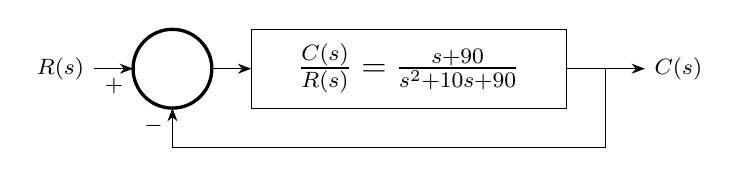
\begin{tikzpicture}[font=\footnotesize]
    \draw[-Stealth] (1,0) node[left]{$R(s)$} -- (1.5,0) node[below left]{$+$};
    \filldraw[color=black, fill=white, very thick] (2,0) circle (.5);
    \draw[-Stealth] (2.5,0) -- (3,0);
    \draw (3,0.5) -- (7,0.5) -- (7,-0.5) -- (3,-0.5) -- (3,0.5);
    \draw (5,0) node[]{\large$\frac{C(s)}{R(s)} = \frac{s + 90}{s^2 + 10s + 90}$};
    \draw[-Stealth] (7,0) -- (8,0) node[right]{$C(s)$};
    \draw[-Stealth] (7.5,0) -- (7.5,-1) -- (2,-1) -- (2,-0.5) node[below left]{$-$};
\end{tikzpicture}
\end{document}